\documentclass[11pt, oneside]{article} 
\usepackage{geometry}
\geometry{letterpaper} 
\usepackage{graphicx}
	
\usepackage{amssymb}
\usepackage{amsmath}
\usepackage{parskip}
\usepackage{color}
\usepackage{hyperref}

\graphicspath{{/Users/telliott/Github/figures/}}
% \begin{center} \includegraphics [scale=0.4] {gauss3.png} \end{center}

\title{Pythagorean Theorem}
\date{}

\begin{document}
\maketitle
\Large

\label{sec:pythagorean_thm}

The most famous theorem of Greek geometry is also the most useful in Calculus.  
\begin{center} 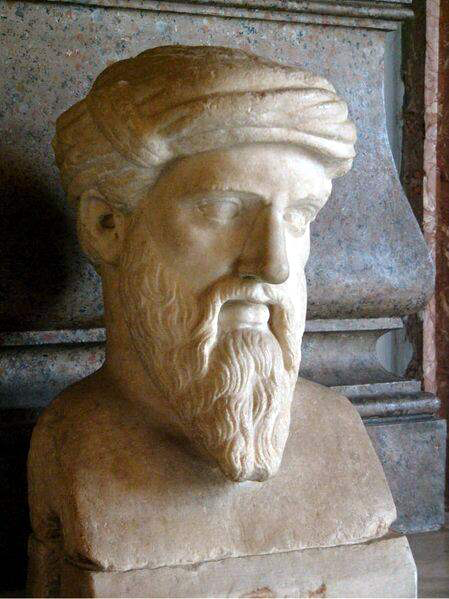
\includegraphics [scale=0.2] {pythagoras.png} \end{center}

Pythagoras (c.570-c.495 BC) was much younger than Thales but may have encountered him as a young man.  Like many other Greek mathematicians, Pythagoras was not from the mainland, but from one of the islands, in his case, Samos, which is not far from Miletus, where Thales lived.  

Pythagoras was famous as a philosopher as well as a mathematician.  In fact, he founded a famous "school" and it is not sure now which of the theorems developed by this school are due to Pythagoras, and which to his disciples.  It is not even clear whether the Pythagorean theorem, as we know it, was known to Pythagoras.

However, it's pretty certain that they knew something.  The $3,4,5$ right triangle and many other Pythagorean triples (see below) had been known for a thousand years (since 1500 BC).  Here is a special case, easily proved, for an isosceles right triangle.

\begin{center} 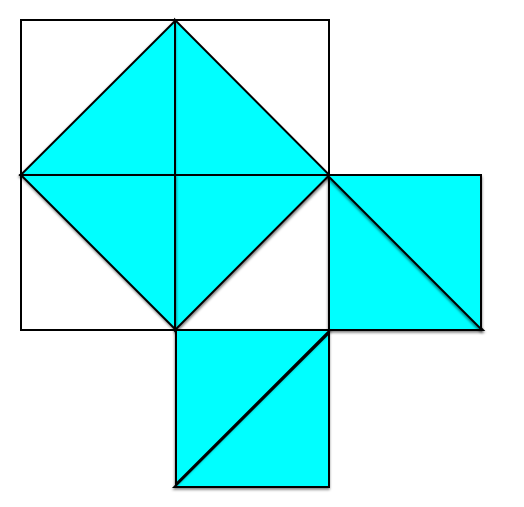
\includegraphics [scale=0.3] {pyth7.png} \end{center}

The area of the square on the hypotenuse is equal to twice the area on each side.

There are literally hundreds of proofs of the general theorem, that if $a$ and $b$ are the shorter sides of a right triangle and $c$ is the hypotenuse, then
\[ a^2 + b^2 = c^2 \]

This one is sometimes called the "Chinese proof."  I can easily imagine proceeding from the figure above to this one by simply rotating the inner square.

\begin{center} 
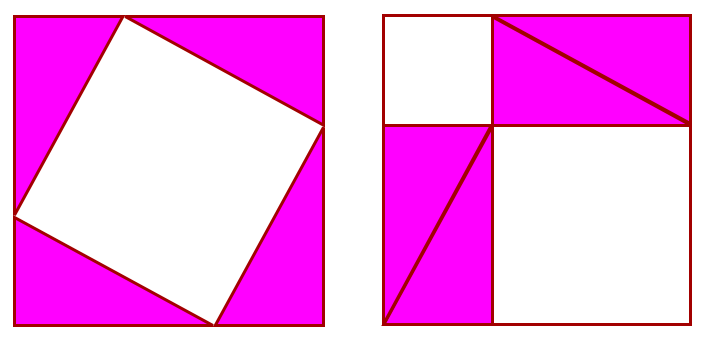
\includegraphics [scale=0.25] {pythagoras1.png} 
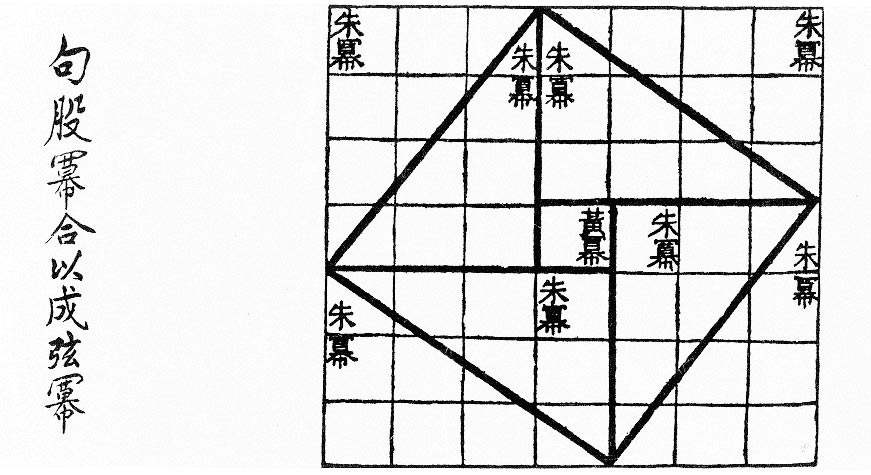
\includegraphics [scale=0.25] {Chinese_pythagoras.jpg}
\end{center}

It really needs no explanation, but ..

In the left panel we have a large square box that contains within it a white square, whose side is also the hypotenuse of the four identical right triangles contained inside.  Altogether the four triangles plus the white area add up to the total.

We simply rearrange the triangles.  Now we evidently have the same area left over from the four triangles, because they still have the same area and the surrounding box has not changed.  

But clearly, now the white area is the sum of the squares on the second and third sides of the triangles.  Hence the two white squares on the right are equal in area to the large white square on the left.  $\square$

This proof is contained in the Chinese text Zhoubi Suanjing (right panel, above).

\url{https://en.wikipedia.org/wiki/Zhoubi_Suanjing}

\subsection*{Euclid's proof}
\begin{center} 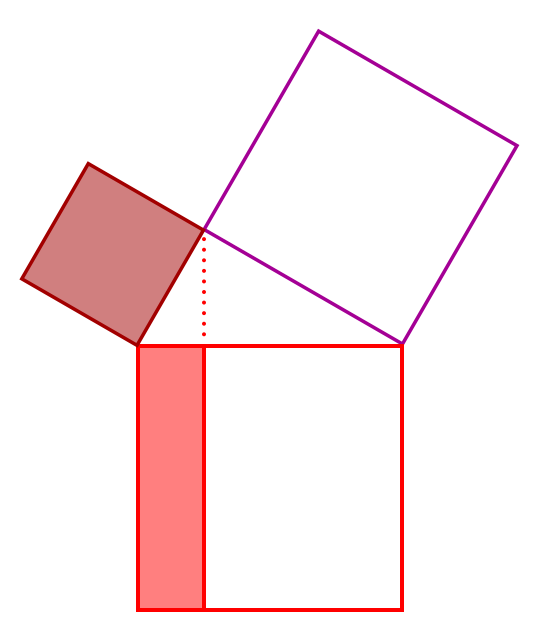
\includegraphics [scale=0.3] {pythagoras2.png} \end{center}

My favorite proof relies on the construction above (Euclid $I.47$, sometimes called the "bridal chair" or the "windmill"), where the central triangle is a right triangle, and the other constructions are squares.  It is a bit more detailed, but it is a gem of a proof, from Euclid, which is a justification for including it.

What we will show is that the part of the large square in red is equal in area to the entire small square, in maroon.

We label some points as shown:
\begin{center} 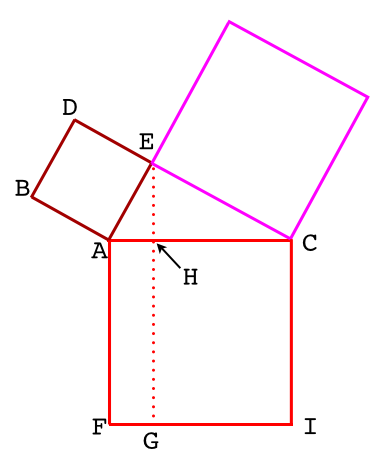
\includegraphics [scale=0.45] {pythagoras3.png} \end{center}
   
First, drop a vertical line $EHG$, constructing the rectangle $AFGH$.
   
Finally, sketch dotted lines for the long sides of two triangles:
\begin{center} 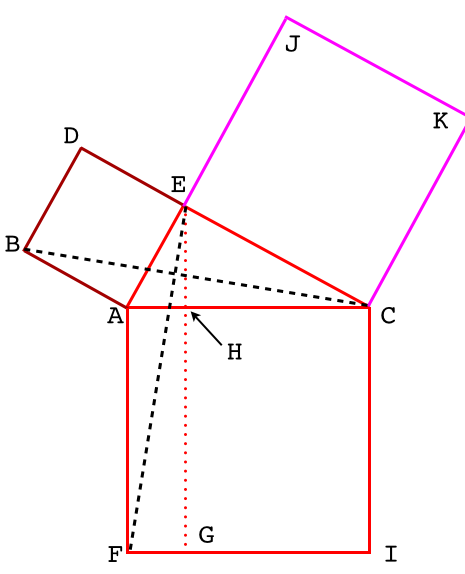
\includegraphics [scale=0.4] {pythagoras4.png} \end{center}

The crucial point is this:  we will show that triangle $\Delta ABC$ is congruent to triangle $\Delta AEF$.  

Use side-angle-side (SAS).  The two sets of sides are evidently equal 
\[ AB = AE, \ \ \ \ AC = AF \]
because these are given as sides of two squares.

What about the included angle?  The angles $\angle BAC$ and $\angle EAF$ each contain a right angle plus the shared angle $\angle EAC$.  So they are themselves equal, and thus we have proved SAS and thus the congruence relationship:
\[ \Delta ABC = \Delta AEF \]

The next part of the proof is to tilt triangle $\Delta ABC$ to the left and see that it has base $AB$ and altitude $AE$ so its area is one-half that of the small square $ABDE$.  On the other hand triangle $\Delta AEF$ has base $AF$ and altitude $AH$ (as well as $FG$) so its area is one-half that of the rectangle $AFGH$.

Hence we have proved that the two colored areas in this figure are equal:

\begin{center} 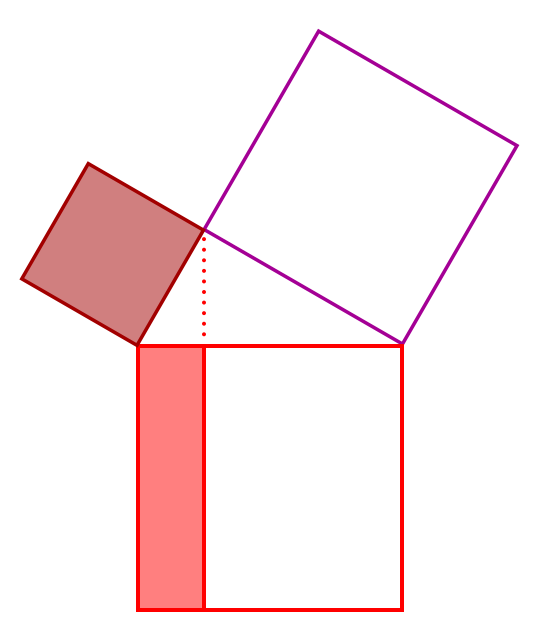
\includegraphics [scale=0.35] {pythagoras2.png} \end{center}
Finally, we could proceed to do the same thing on the right side of the figure, but we just appeal to symmetry.  All the equivalent relationships will hold.  

$\square$

There are several hundred proofs of the Pythagorean theorem.  Many of them are algebraic.  Here is a classic:

\begin{center} 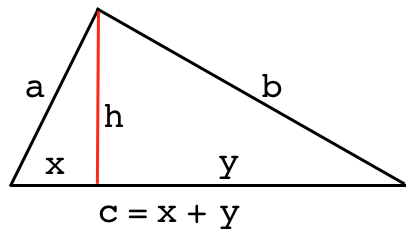
\includegraphics [scale=0.4] {triangle3.png} \end{center}

We know that when an altitude is drawn in a right triangle, the two resulting right triangles are similar (use complementary angles if you need to convince yourself again).  So we have equal ratios of sides.  Here are two sets:

hypotenuse to short side
\[ \frac{a}{x} = \frac{b}{h} = \frac{c}{a} \]
hypotenuse to long side
\[ \frac{a}{h} = \frac{b}{y} = \frac{c}{b} \]

From the first
\[ a^2 = cx \]
From the second
\[ b^2 = cy \]
Just add
\[ a^2 + b^2 = cx + cy \]
\[ = c(x+y) = c^2 \]

\subsection*{Garfield}

There is one by a future President of the United States, James A. Garfield.  (He was a congressman at the time).

\begin{center}
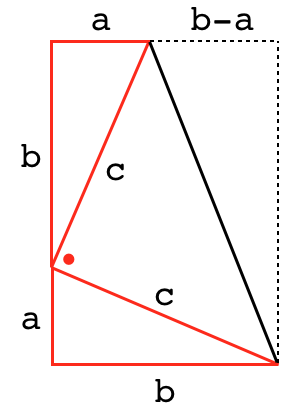
\includegraphics [scale=0.5] {garfield4.png}
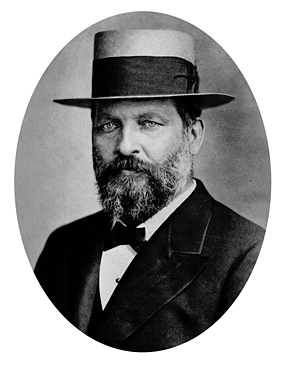
\includegraphics [scale=0.5] {garfield2.png}
\end{center}

Draw a right triangle and a rotated copy as shown.  The angles opposite sides $a$ and $b$ are complementary angles.  So the angle marked with a dot is a right angle, and the triangle with sides labeled $c$ is a right triangle.

The area of the quadrilateral is the product of the side $(a + b)$ and the \emph{average} of $a$ and $b$ (top and bottom).  This can be seen intuitively.  The halfway point of the solid red line has horizontal dimension $(a+b)/2$.  Hence
\[ A = (a+b) \cdot \frac{1}{2} (a + b) \]

If you're worried about that argument, just subtract the area of the triangle with two dotted sides from the quadrilateral that includes it:
\[ A = (a + b)b - \frac{(a+b)(b-a)}{2} \]
\[ = (a + b)(b - \frac{b}{2} + \frac{a}{2}) \]
\[ = (a+b) \cdot \frac{1}{2} (a + b) \]
which is just what we said.  So now:
\[ = \frac{a^2}{2} + ab + \frac{b^2}{2} \]

But we can also calculate the area of the quadrilateral as the sum of the three triangles:
\[ A = \frac{ab}{2} + \frac{ab}{2} + \frac{c^2}{2} \]
Equate the two and the result follows almost immediately.

$\square$
 
\subsection*{Corollary}
There are several important corollaries of the Pythagorean theorem.  We'll derive one later called the law of cosines.  Here is another from the Islamic geometer Ibn Quorra, who brought algebraic techniques, shunned by the Greeks, to geometry.
\begin{center} 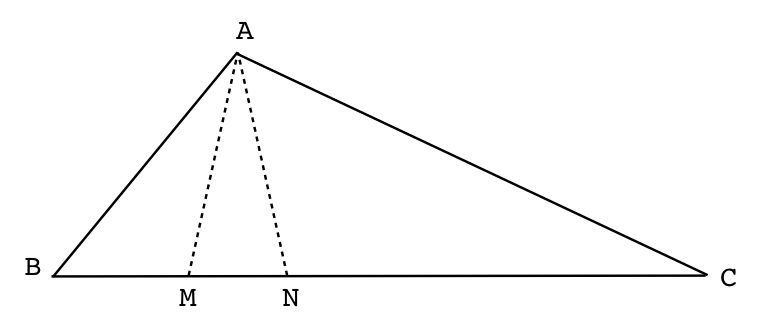
\includegraphics [scale=0.4] {pyth_corollary.png} \end{center}

Let $\triangle ABC$ be \emph{any} triangle (here it is obtuse).  Draw $AM$ and $AN$ so that the new angles $\angle AMB$ and $\angle ANC$ are equal to $\angle A$.  The corresponding triangles are similar to the original, because they share the angle of measure $A$ plus one other from the original triangle.

Then
\[ BM:AB = AB:BC \]
Thus, $AB^2 = BM \times BC$.  Similarly
\[ NC:AC = AC:BC  \]
So $AC^2 = NC \times BC$
Therefore
\[ AB^2 + AC^2 = BM \times BC + NC \times BC \]
\[ = (BM + NC) \times BC \]

In the case where the angle at vertex $A$ is a right angle, then $M$ coincides with $N$, and $BM + NC = AC$, and this reduces to the Pythagorean theorem.

\subsection*{geometric mean}

As a slight detour from calculus, but on the topic of this chapter

\begin{center} 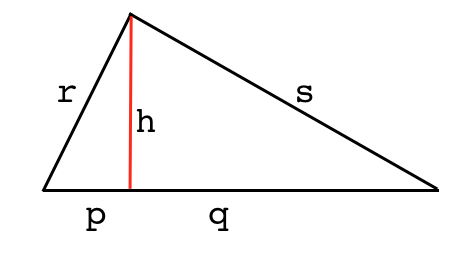
\includegraphics [scale=0.4] {pythagoras6.png} \end{center}

We will show that
\[ h^2 = pq \]
\[ h = \sqrt{pq} \]
That is, $h$ is the geometric mean of these two values $p$ and $q$.

Proof.

Using the Pythagorean theorem with the two small triangles (also right triangles), we obtain:
\[ h^2 + p^2 = r^2 \]
\[ h^2 + q^2 = s^2 \]
Summing
\[ 2h^2 + p^2 + q^2 = r^2 + s^2 \]

Using the theorem with the big triangle:
\[ r^2 + s^2 = (p + q)^2 \]
\[ = p^2 + 2pq + q^2 \]

Equating the two expressions for $r^2 + s^2$ we get:
\[ 2h^2 + p^2 + q^2 = p^2 + 2pq + q^2 \]
 \[ h^2 = pq \]
 \[ h = \sqrt{pq} \]
 
\end{document}